\chapter{De Bruijn Graphs}

In this chapter, we discuss de Bruijn graphs, which are important tools
for handling short reads and serve as a foundation for many assembly algorithms.
We will discuss definition and construction of de Bruijn graphs,
techniques for handling sequencing errors and then we will show several
options for handling paired reads. In the end we will show another
application of de Bruijn graphs as a tool for correcting long read with high error
rate by short reads with low error rate.

\bigskip

A de Bruijn graph \citep{de1946combinatorial} is a structure for representing
overlaps between strings.

\begin{definition}[De Bruijn graph]
A De Bruijn graph is directed graph. 
For given $k$, vertices of de Bruijn graph represent sequences of length $k$
($k$-mers). The edges of de Bruijn graph represent possible overlaps of length $k-1$, i. e. 
if have have an edge $(u, v)$ and vertex $u$ represents $k$-mer $a_1, a_2, \dots, a_k$, then
vertex $v$ represents $k$-mer $a_2, a_3, \dots, a_k, x$ and $k$-mer in vertex $v$ can
follow $k$-mer in vertex $u$.
\end{definition}

Besides application in DNA sequencing, de Bruijn graphs are used
in design of fault tolerant networks \citep{ftndeb} and 
distributed hash tables \citep{koorde}.

\section{De Bruijn Graphs for Sequence Assembly}


De Bruijn graphs used for sequence assembly
\citep{pevzner2001eulerian,Velvet} have few modifications
to accomodate for possibility of reads coming from both strands of DNA.

For each vertex $v$ there is a twin vertex $v^{'}$ which
represents reverse complemented $k$-mer. Union of $v$ and $v^{'}$ is called a block.
During manipulation of De Bruijn graph any change applied to node $v$ is also symetrically
applied to its twin $v^{'}$.
To ensure that some $k$-mer is not the same as its reverse complement, $k$ must be an odd number.

Vertices $u$, $v$ in the de Bruijn graph can be connected by directed arcs if the last
$k-1$ bases of $u$ are same as the first $k-1$ bases in $v$. Also note that
if there is an edge between vertices $u$, $v$, there is an inverted edge between their twins,
i.e. there is an edge from $v^{'}$ to $u^{'}$.

We construct De Bruijn graph from reads in a straighforward way.
We extract every $k$-mer from each read and its reverse complement.
Then we join by edge each pair of $k$-mers which are consecutive in some read.
Some assemblers also record simple statistics that will be useful in later
stages of the assembly process, such as multiplicity of each vertex or edge.

This construction can be done in efficient way by using hash tables, like in Velvet \citep{Velvet}.
There are also space-efficient representations of De Bruijn graphs based on Bloom filters \citep{minia}.

\begin{figure}
  \centerline{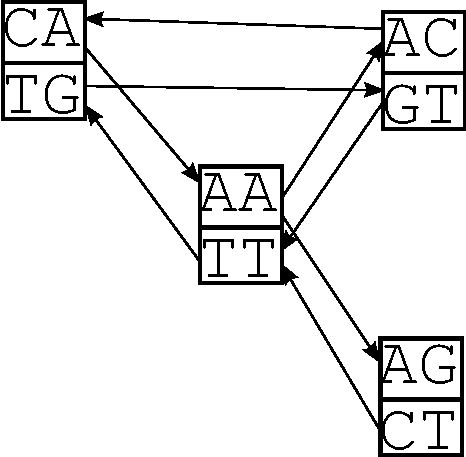
\includegraphics[scale=0.5]{../figures/db.pdf}}
  \caption{Example of de Bruijn graph constructed from reads: \texttt{AACA}, \texttt{CTTG}, with $k=2$.}
\end{figure}

After constructing de Bruijn graph the assembly can be represented
as a set of walks in de Bruijn graph. Different assemblers
have different criteria on optimal set of walks in de Bruijn graph. 

One approach is to look for Eulerian path through graph.
Even better approach is to look for
Eulerian superpath -- the path which visits every read, i.e. if some read
is broken into vertices $v_1, v_2, \dots, v_n$, then the Eulerian superpath
should contain $v_1, \dots, v_n$ as subpath.

\begin{definition}{Eulerian superpath problem.}
Given graph $G$ and set of paths $\mathbb{P}$ find path $P$, which contains
every path from $\mathbb{P}$ as subpath.
\end{definition}

Euler assembler \citep{pevzner2001eulerian})solves some instances of Eulerian superpath problem
using simple transformations which transform Eulerian superpath instance to equivalent Eulerian path instance.

Other assemblers like Velvet \citep{Velvet} just join vertices which can be joined
unambiguosly, i.e. they join vertices $u$, $v$ is there is an edge from $u$ to $v$ and
it is only edge comming out of $u$ and only edge comming into $v$. After this joining
each vertex represents one contig of the assembly.

\subsection{Handling Sequencing Errors}

\begin{figure}
  \centerline{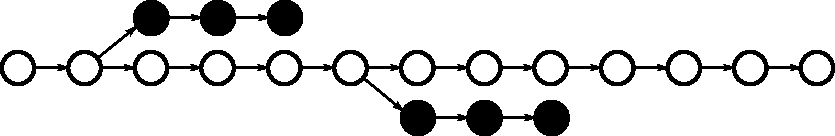
\includegraphics[scale=0.9]{../figures/tips.pdf}}
  \caption{Example of two tips (in black).}
  \label{fig:tips}
\end{figure}

\begin{figure}
  \centerline{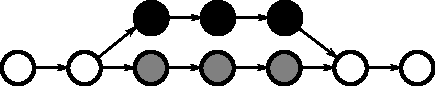
\includegraphics[scale=0.9]{../figures/bubble.pdf}}
  \caption{Example of bubble with two paths marked in black and gray.}
  \label{fig:bubble}
\end{figure}

Sequencing errors in reads increase complexity of the de Bruijn graph
\citep{pevzner2001eulerian}. The common artefacts in a graph that
appear due to sequencing errors are tips and bubbles
(see Fig. \ref{fig:tips}, \ref{fig:bubble}). Assemblers like Velvet \citep{Velvet}, ABySS \citep{Abyss} handle
errors directly during the construction of de Bruijn graph by detecting these artefacts
and removing them.

The naive approach would be to remove all $k$-mers with low coverage.
This can be problematic since some sequencing technologies do not produce reads with uniform coverage
and consequently we would remove good low coverage regions and consequently the graph would become disconnected.
Instead several more sophisticated techniques have been proposed to remove
most of the artefacts in de Bruijn graph.

\paragraph{Removing tips.} A tip is chain of vertices disconnected at one end. 
Tips usually represent some local errors in the reads. Their removal is pretty straighforward
and removing them does not destroy connectivity in the graph. But sometimes the tips
could represent correct sequence interupted by a gap in the coverage.
Velvet \citep{Velvet} removes tips, which are at most $2k$ bases long and the edge starting
the tip has lower multiplicity that some other edge in the branching vertex.

\begin{figure}
  \centerline{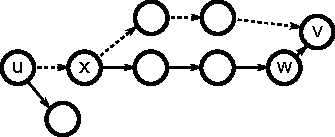
\includegraphics[scale=0.9]{../figures/bubblefind.pdf}}
  \caption{Example of bubble finding. We start search from node $u$. Shortest path between
$u$ and $v$ is shown using dashed edges. When searching node $w$ we will visit node
$v$ again. Now we can find closest common ancestor of current path to $w$ and shortest path to $v$,
which is vertex $x$.}
\label{fig:bubblerem}
\end{figure}

\paragraph{Removing bubbles.} Bulles are two or more paths which share start and end vertices
and contain similar sequences.
Such bubbles are typically caused by small error in the middle of the read.
Velvet finds such similar paths using the following algorithm:
It starts breadth first search like algorithm from an arbitrary vertex, but considers higher converage
arcs as shorter. Whenever it encounters previously visited vertex $v$ it tries to find closest common ancestor
of the current path and shortest path to $v$ (see Fig. \ref{fig:bubblerem}). Then it extract
sequences belonging to both paths and
if these two paths are judged to be similar enough, the longer path is merged into the shorter one. 
 
\bigskip

Other option is to use tools like QUAKE \citep{Quake}, which try to correct reads
without assembling them. This tools usualy consider $k$-mers with low abundance
as errornous and try to correct them using few simple edits in reads.

After correcting for errors, we usually simplify de Bruijn graph by joining vertices
with unambiguous connection as mentioned above. 
We can use this vertices as a base for forming contigs of the assembly.
Most assemblers goes further and use various heuristics
to incorporate information from long and paired reads.
In the next section we will look more into handling paired reads.

\section{Handling Paired Reads}

De Bruijns graphs do not incorporate any information from paired reads.
In this chapter we describe two options for incorpoating this information:
heuristic postprocessing and paired e Bruijn graphs.

\subsection{Heuristic Postprocessing for Paired Reads}

ABySS \citep{Abyss} uses paired reads in the following way:
After initial error correction in De Bruijn graph, we align paired reads
to reasonably long vertices in De Bruijn graph. Two vertices are considered linked
if there are at least $p$ read pairs (usually $p=5$) which join the vertices.
We denote $P_i$ the set of vertices which are linked to vertex $v_i$.
Then we perform search for single unique path from $v_i$ through De Bruijn graph which visits
each vertex from $P_i$. We usualy limit this search by estimated distance from $v_i$ to each element
from $P_i$. This process is performed for each vertex and final consistent paths
are stitched to final assembly.

Allpaths assembler \citep{allpaths} uses more complicated approach.
It requires at least two Illumina short read libraries -- one with short insert size
(around $100$ - $200$ bases) and one with medium insert size (around $3000$ bases).
Their main idea is to find all possible fillings of the gap in the middle of paired read
using using other reads (without regard to their pairing)
having some minimum overlap K with each other, via a process of “walking” from
one read to the other. Then they merge these filled reads to produce assembly. 

To reduce computational complexity of this approach they split assembly problem
into several regions and assemble them separately in process called localization.
Localization starts by building de Bruijn graph of the assembly and building initial
contigs from it. Then we select long enough contigs as seeds. 
The region of an assembly is build from seed, its neighbourhood (everything
in 10000 bases around the seed) and all reads from the neighbourhood.
We assemble each region separetely and then merge result into final assembly.

\subsection{Paired de Bruijn Graphs}

\citet{Paired} argues that heuristic postprocessing
usually works well is simple cases, but fails when assembly contains
several repeated regions after each other.

He introduces concept concept of paired De Bruijn graphs to incorporate paired read
information directly into the de Bruijn graph.
In the following we will present the construction of 
paired de Bruijn graph.
For simplicity, we will ignore reverse complements and problems associated with that.

\paragraph{Paired de Bruijn graphs with exact insert sizes.}
Let $k$-bimer be a pair of two $k$-mers $(a, b)$. Each vertex 
represents one $k$-bimer and edges represent
consecutive $k$-bimers similarly as in an ordinary de Bruijn graph. 
From each pair of reads, we will produce $k$-bimers in a straighforward way:
$i$-th $k$-bimer will be created using the $i$-th $k$-mer from the first read and 
the $i$-th $k$-mer from the second read.
Edges in the graph are given by consecutive pairs of $k$-mers from reads.

For example if we had paired read $ACCTG, TCGAT$ and $k = 3$, then our
$k$-bimers would be: $(ACC, TCG), (CCT, CGA), (CTG, GAT)$ and each consecutive bimers
would be joined by edge.

To create the assembly we can use same methods as in ordinary de Bruijn graphs
(euler paths or joining umambigously connected vertices).

\paragraph{Paired de Bruijn graphs with approximate insert sizes.}
Lets assume that insert sizes are from the interval $d \pm \Delta$.
We start by constructing paired de Bruijn graph described in previous paragraph.
The key insight is that if two $k$-bimers $(a, b)$ and $(a, b^{'})$ come from
the same location of $a$ then the distance of $b$ and $b^{'}$ in the ordinary De Bruijn graph is at
most $2\Delta$.

Consequently, in the next step we will merge all vertices $(a, b)$, $(a, b^{'})$ if there is a path
between $b$ and $b^{'}$ in ordinary De Bruijn graph with length at most $2\Delta$.
Note that sometimes me might merge vertices which do not belong to the same location of the original DNA
sequence, but if two bimers belong to the same location of the original DNA sequence, we will merge
them (if there is a sufficient coverage of sequencing).

\bigskip
Like in the case of ordinary de Bruijn graph we need to deal with errors in reads
and also with insert size outliers. This approach still cannot handle multiple
read libraries with various insert sizes and combination of paired libraries and long reads.
One implementation of this approach is SPAdes assembler \citep{Spades}.


\section{Correction of Long Reads with High Number of Errors}

PacBio if a new technology used to sequence DNA that produces
rather long reads (up to 20000 bases and more) but with many errors
($15\%$ error rate). There is a need to correct these errors in a reasonably
efficient way. Constructing de Bruijn graph directly from PacBio reads
cannot lead to anything usefull since we can expect one of every six bases to be
incorect, so standard correction techniques for de Bruijn graph cannot be applied.
Also directly applying overlap-layout-consensus framework is not a good idea, since
with such high error rate we can expect many false positives in overlaps.

One way to correct PacBio reads is to align them to each other and use that for self correction.
This was done by \citet{MHAP}. But this approach requires high coverage
of PacBio reads, which can be cost a lot.

Other way to do so this to correct Pacbio reads using shorter reads with smaller
error rate. There are approaches which directly map short read on long reads like
PacbioToCA \citep{PacbioToCA}. Their downside is that this mapping step
is computationally very expensive.

One way to speed up this mapping step is to first generate De Bruijn graph from short reads
and then attempt to map long reads to paths in this graph.
This was implemented in LoRDEC \citep{Lordec}.
The benefit of this approach is that in the former
case there were many short reads mapped to similar location of the long read, in this
case there are only few paths mapped to same location of the long read. In other
words we might expect speedup proportional to the coverage of the short read sequencing.

More specifically, after construction the of de Bruijn graph, we remove all vertices
with very low coverage (to keep $k$-mers unlikely containing errors). The $k$-mers belonging
to the de Bruijn graph are called solid, the others are called weak.
Then we split each long read into $k$-mers.
Each solid $k$-mer from long read is considered to be correct. 
Our goal now is to correct regions between solid $k$-mers. To do so, we are trying
to find a path through de Bruijn graph which minimizes edit distance between the path
and the region of the sequence.

\section{Summary}

We defined de Bruijn graph as a graph holding $k$-mers and overlaps between
them. The typical graph formations which arise from sequencing errors are
tips and bubbles, which could be removed from the graph. To handle paired reads
we can either use heuristical postprocessing or paired de Bruijn graphs. 
There are also more application of de Bruijn graphs in processing of DNA data.
The example is using them to correct long reads with high error rate.
